% ==============================================================================
\chapter{Pixel-beam telescope and simulation framework}
\label{ch:Telescope}
%==============================================================================  

%% --------------------------------------------- %%
\section{The Timepix3 telescope} \label{sec:Timepix3Telescope}
The Timepix3 telescope is used as a beam reference telescope and is
shown in Figure~\ref{fig:TPX3Telescope}. The telescope is used to
reconstruct the tracks of the particles going through its planes and
extrapolate the position on the Device Under Test (DUT). This allows
to compare the position of the hit on the DUT with the reconstructed
track and calculate the position, time resolutions and the efficiency
of the device. The Timepix3 telescope is made of 6 planes of Timepix3
ASICs~\cite{Timepix3_Poikela} bump bonded to $300\,\micron$ thick
p-in-n planar sensors. The planes are rotated by $9\degrees$ around
the x axis (perpendicular to the beam axis) and the z axis (parallel
to the beam axis) to optimise the charge sharing within the sensors
and obtain a pointing resolution of $\sim$$2\,\micron$ on the device
under test (DUT). The data-driven zero-suppressed mode is used for the
data acquisition of the Timepix3 readout ASICs.

\begin{figure}[htbp]
  \centering
  \begin{tikzpicture}
    \node[anchor=south west,inner sep=0] (image) at
    (0,0){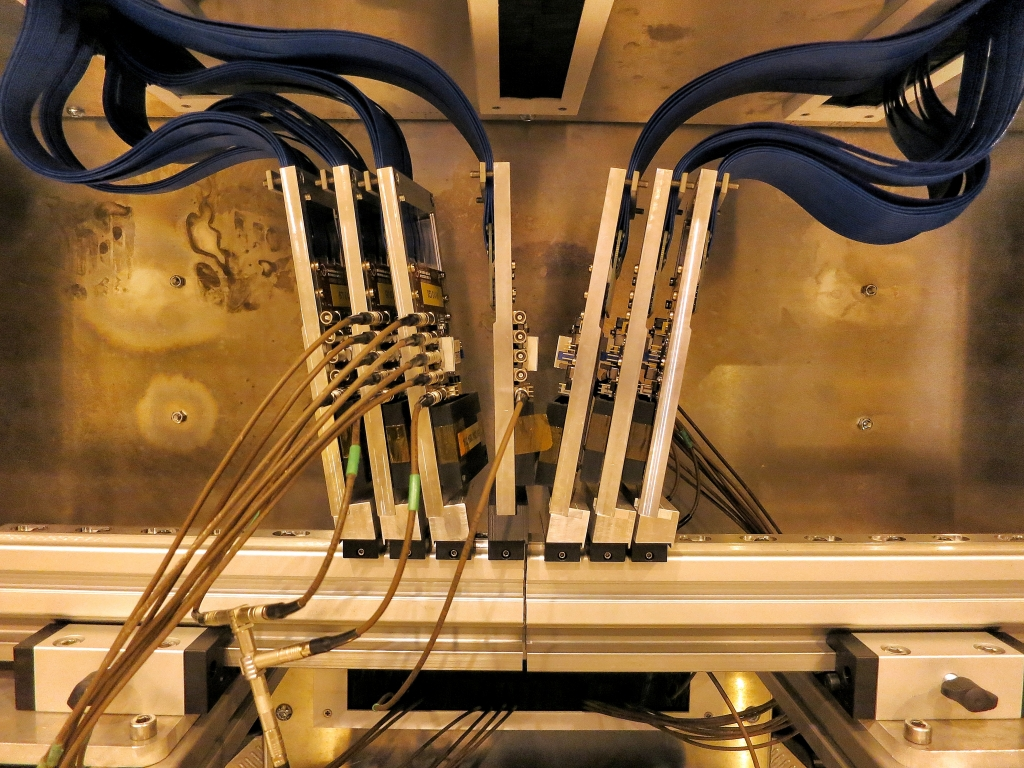
\includegraphics[width=0.6\textwidth]{ActiveEdge/Timepix3Telescope.jpeg}};
    \begin{scope}[x={(image.south east)},y={(image.north west)}]
      \node[above, color=white] at (0.5, 0.85) {Device Under Test};
      \node[above, color=white] at (0.5, 0.78) {(\textbf{DUT})};
    \end{scope}
  \end{tikzpicture} 
  \caption{The Timepix3 beam reference telescope.}
  \label{fig:TPX3Telescope}
\end{figure}
%% --------------------------------------------- %%
\section{Reconstruction software}
\subsection{EUTelescope}
The EUTelescope software~\cite{Rubinskiy} is used to reconstruct the
telescope tracks and analyse the telescope data. It is based on the
ILCSoft framework (REF?). Using a pipeline of Marlin
processors~\cite{Gaede:2006pj}, it allows to convert the raw data to a
ROOT (REF?) format and with the intermediate steps in the LCIO (REF?)
format. The reconstruction chain is defined in the steps below:

\begin{enumerate}
\item Converter: converts the raw files written by each telescope
planes and the DUT in a binary format to an LCIO event. The
data-driven zero-suppressed mode is used for the data acquisition of
the Timepix3 readout ASICs. This mode allows for a very low dead-time
and all the particles at the SPS spill are recorded. Every hit is
written with a 64-bit time-stamp (\texttt{long long int}) related to
the TOA (time-of-arrival). The hits written in the raw file are not
necessarily ordered in time. In the converter processor, the hits
within a timing window of 3~ms are read and filled into a vector. The
hits in the vector are ordered in time according to their time
stamps. An LCIO event is built by choosing the hits in the six
telescope planes and the DUT with time stamps differing by
$2.5\,\microsecond$. With this constraint, most probably one track per
event is obtained.
Hot pixels (with the maximum allowed frequency of 0.1) are as well
calculated and also the $\eta$-correction~\cite{Belau:1983eh} values.

\item Clustering: the clusters in each plane is found.
\item Hit making: reconstruction of the hit position for each cluster
with the $\eta$-correction method.
\item Alignment: by assuming straight tracks, the alignment processor
uses Millepede~II algorithm~\cite{Blobel20065} to align the telescope
planes with respect to each other. It consists of a least squares
minimisation problem ($\chi^2$minimisation). A proper definition of
the geometry is important.
\item Track finding: fits the tracks based on the hits on the
telescope planes with taking to account the multiple scatterings
(radiation length of the material for the described geometry),
positions of the planes. The \texttt{EUTelTestFitter} algorithm is used for the
analysis of the test-beam. (TO PUT SOME CHI2 DISTRIBUTION PLOTS). The
tracks are then extrapolated on the DUT.
\end{enumerate} 

\subsection{pyEudetAnalysis}
For the analysis of the DUT data, the python-based software
\texttt{pyEudetanalysis} is used. It can be found as a GitHub directory~\cite{pyeudet}.



%% --------------------------------------------- %%
\section{AllPix: a \textsc{Geant4}-based simulation software}
AllPix~\cite{allpix}, is used as a wrapper on \textsc{Geant4} to
simulate the test beam setup. The software is written in C/C++. It
provides a flexible interface to define the geometry of the
setup. \cref{fig:TPX3TelescopeAllpix} shows the telescope planes
and the DUT simulated in AllPix.

\begin{figure}[htbp]
  \centering
  \begin{tikzpicture}
    \node[anchor=south west,inner sep=0] (image) at
    (0,0){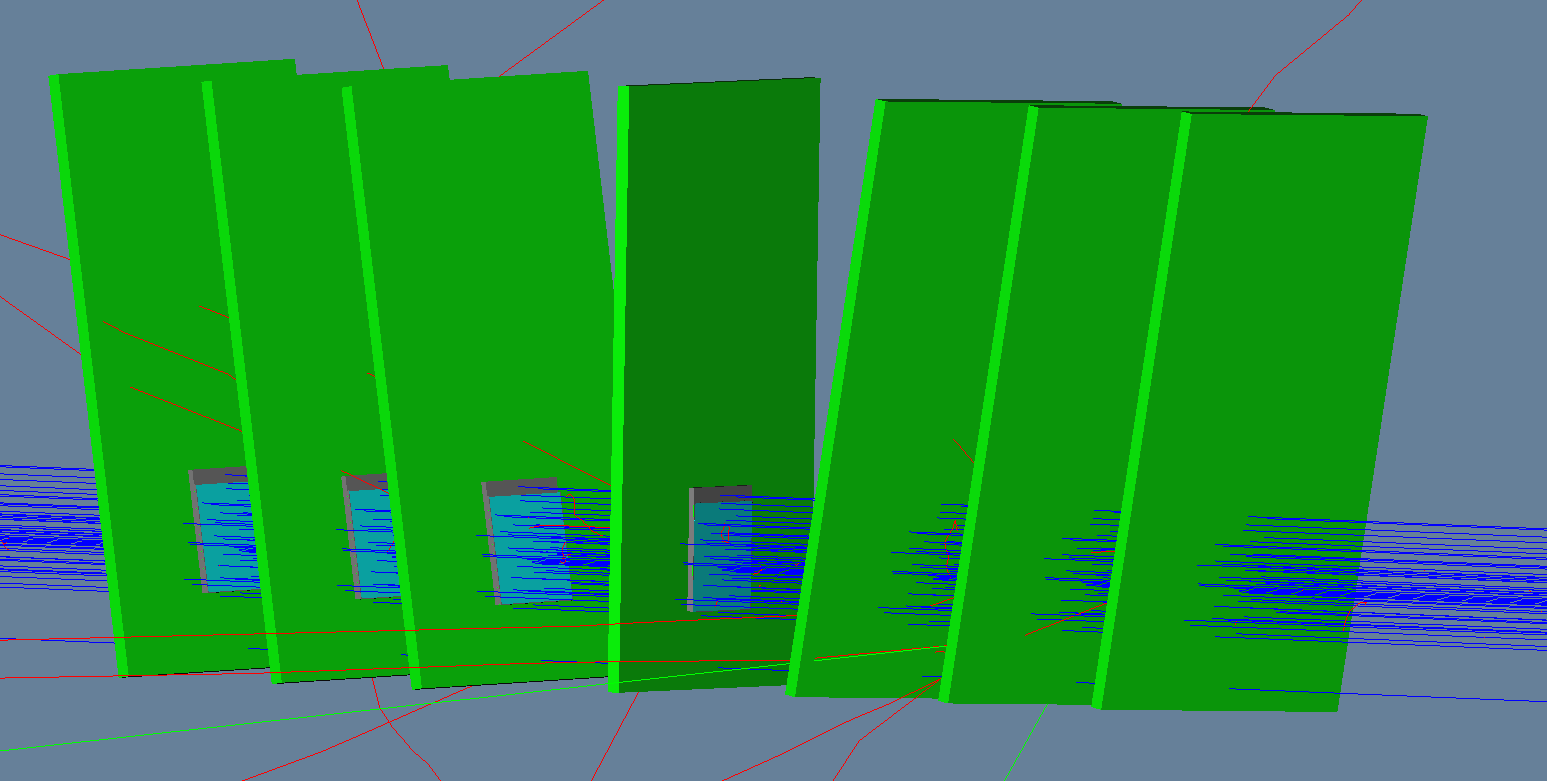
\includegraphics[width=0.8\textwidth]{figures/ActiveEdge/Allpix_telescope_withParticles.png}};
    \begin{scope}[x={(image.south east)},y={(image.north west)}]
      \node[above, color=white] at (0.45, 0.65) {\textbf{DUT}};
    \end{scope}
  \end{tikzpicture}
  \caption{Simulation of the Timepix3 telescope with AllPix.}
  \label{fig:TPX3TelescopeAllpix}
\end{figure}

The main components of the software are described here-below:
\begin{enumerate}
\item Digitiser: \textsc{Geant4}, for each simulation step
  (\texttt{G4Step}) through the matter, provides the energy deposited
  in the sensitive material. The step length can be customised. For
  thin sensors simulations a step of $2\,\micron$ is selected and
  provides a precise energy deposition. The semiconductor physics in a
  Silicon detector is then defined in the digitiser. The drift and
  diffusion are performed at each step to simulate the electron-hole
  pair movement in the electric and magnetic fields. The readout ASIC
  is also simulated in the digitiser. The electronic noise is added
  and a threshold is applied to the hits. The hit energy is converted to the
  digital value TOT (time-over-threshold) using the readout ASICs calibrations.
\item \texttt{pixeldetector.xml}: defines a pixel detector
(\texttt{<pixeldet id=''300"/>}) with a unique ID. It contains all the
properties of the pixel detector like the pixel pitch, detector
thickness, chip thickness, PCB properties and other geometry
properties related to an assembly. It can be customised and define the
parameters of the digitisers. This will allow to run the program
without needing to compile whenever one wants to change a parameter.
\item \texttt{macro.in}: Define the position of the detectors in the
space by giving the x, y and z position of the centre of the detectors
and the rotations around the x, y and z axes. The physics list used by
\textsc{Geant4} is also defined in this file. Visualisation parameters
are also given. The General Particle Source (GPS), which is the
\textsc{Geant4} toolkit for Monte-Carlo of the high-energy particle
transport is also described in the macro. The particle type, the beam
energy, the position and distributions are customisable. The
simulation is done based on the frames.
\end{enumerate}


\subsection{Coordinate system}

Pixel coordinates (X, Y) and the center of the pixels in \textcolor{blue}{local coordinates (x,
  y)} (in millimeters) in the corners of the sensor. In
\cref{fig:coordinateSystem}, we are looking from the sensor side with
the periphery on the top. The same coordinate system is used for both
AllPix and EUTelescope.
\begin{figure}[htbp]
  \centering
  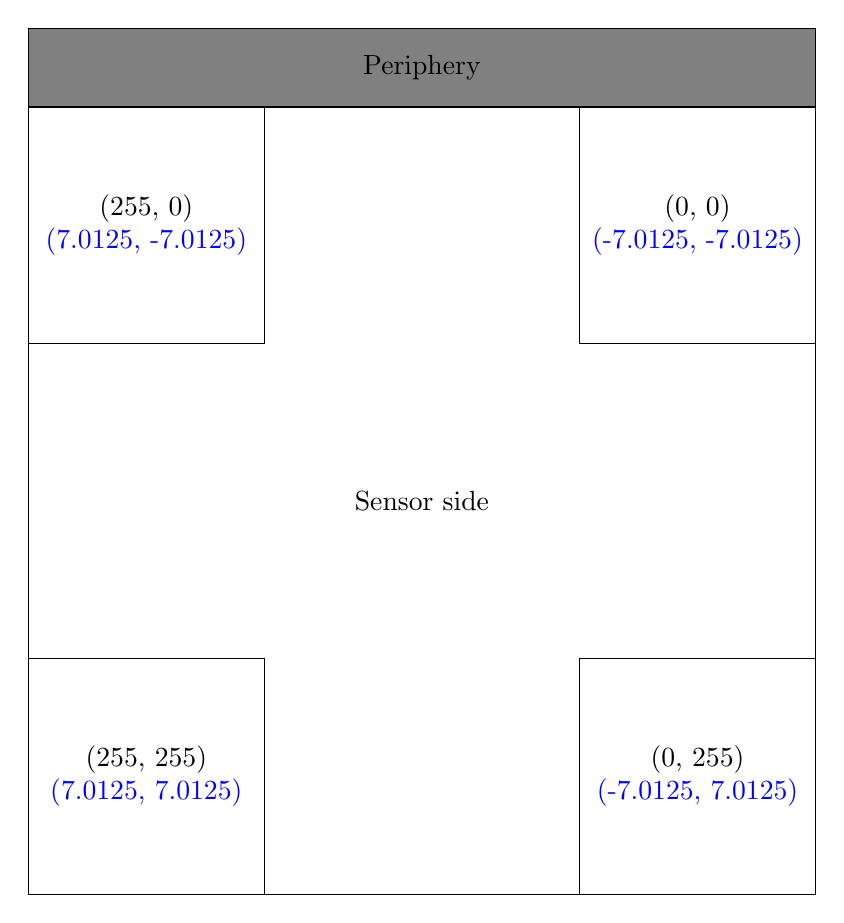
\begin{tikzpicture}
    \begin{scope} 

      \draw (0, 0) rectangle (10, 10) node[pos=.5] {Sensor side};
      \draw[fill=gray] (0, 10) rectangle (10, 11) node[pos=.5]
      {Periphery};

      \draw (0, 10) rectangle (3, 7) node[align=center, pos=.5] {(255, 0) \\ \textcolor{blue}{(7.0125, -7.0125)}};
      \draw (7, 10) rectangle (10, 7) node[align=center, pos=.5] {(0, 0) \\ \textcolor{blue}{(-7.0125, -7.0125)}};
      
      \draw (0, 0) rectangle (3, 3) node[align=center, pos=.5] {(255,
        255) \\ \textcolor{blue}{(7.0125, 7.0125)}};
      \draw (7, 0) rectangle (10, 3) node[align=center, pos=.5] {(0, 255) \\ \textcolor{blue}{(-7.0125, 7.0125)}};
      % \draw[help lines,xstep=.1,ystep=.1] (0, 0) grid (10,10);
      % \foreach \x in {0,1,...,9} { \node [anchor=north] at (\x/10,0) {0.\x}; }
      % \foreach \y in {0,1,...,9} { \node [anchor=east] at (0,\y/10)
      %   {0.\y}; }

    %   \draw[step=2cm,color=gray] (-5, -5) grid (5, 5);
    %   \matrix[matrix of nodes,nodes={inner sep=0pt,text width=2cm,align=center,minimum height=2cm}]{
    %     {(255, 0) \\ \textcolor{blue}{(7.0125, -7.0125)}} & &  & {(0,0) \\ \textcolor{blue}{(-7.0125, -7.0125)}} \\
    %     &  &  &  \\
    %     &  &  &  \\
    %     {(255, 255) \\ \textcolor{blue}{(7.0125, 7.0125)}} &  &  & {(0, 255) \\ \textcolor{blue}{(-7.0125, 7.0125)}} \\};
    \end{scope}  
  \end{tikzpicture}
  \caption{}
  \label{fig:coordinateSystem}
\end{figure}

%% --------------------------------------------- %%
\section{Timepix3 telescope performance}
\label{sec:telescopePerformance}

\subsection{Beam angle}

For MC beam angle distribution:

\begin{equation}
  \phi=arctan{{x_2-x_{DUT}} \over {z_2-z_{DUT}}} \; ,
  \label{eq:beamAnglePhi}
\end{equation}

\begin{equation}
  \theta=arctan{{y_2-y_{DUT}} \over {z_2-z_{DUT}}} \; ,
  \label{eq:beamAngleTheta}
\end{equation}

\begin{figure}[htbp] \centering
  \begin{subfigure}[b]{0.45\textwidth}
    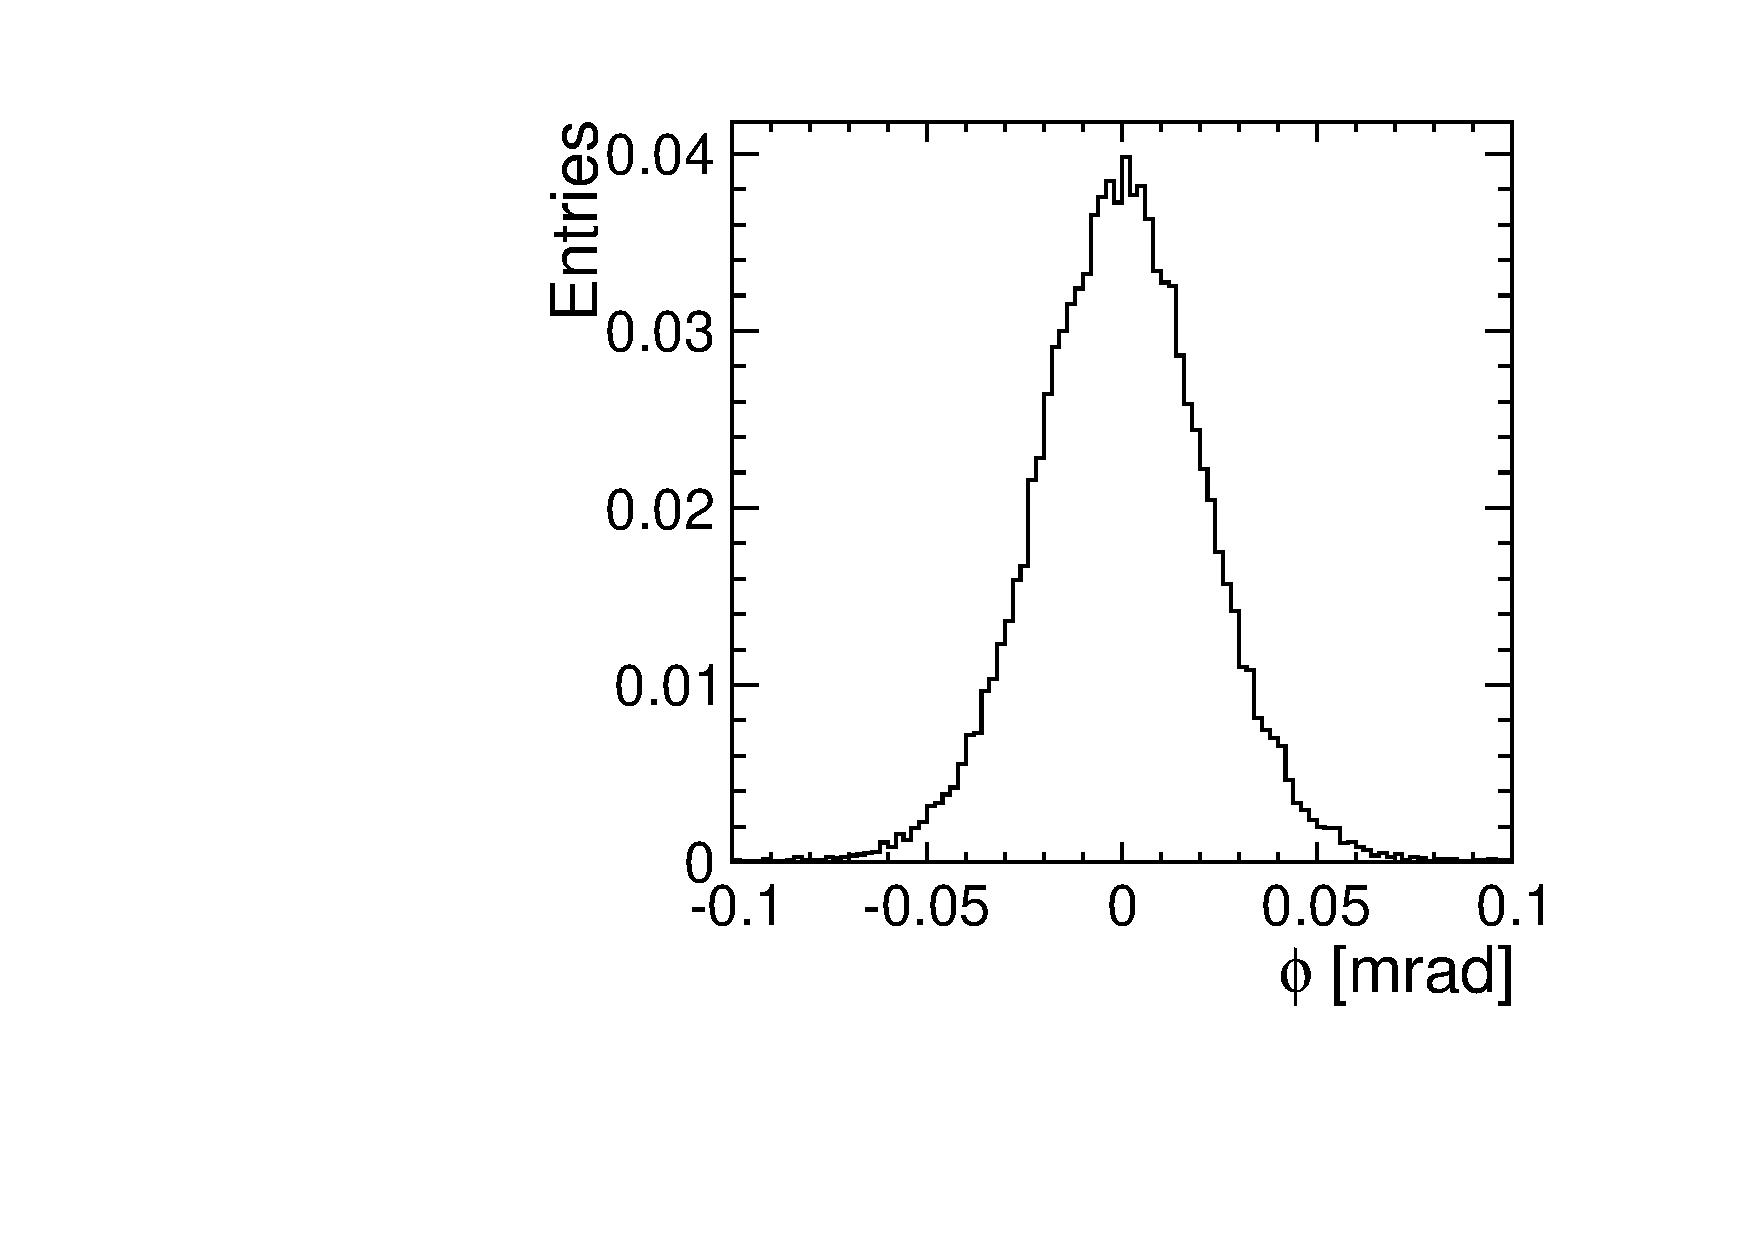
\includegraphics[width=\textwidth]{./figures/Telescope/MC_trackAnglePhi_planes_302_100.pdf}
    \caption{}
  \end{subfigure}\hfill
  \begin{subfigure}[b]{0.45\textwidth}
    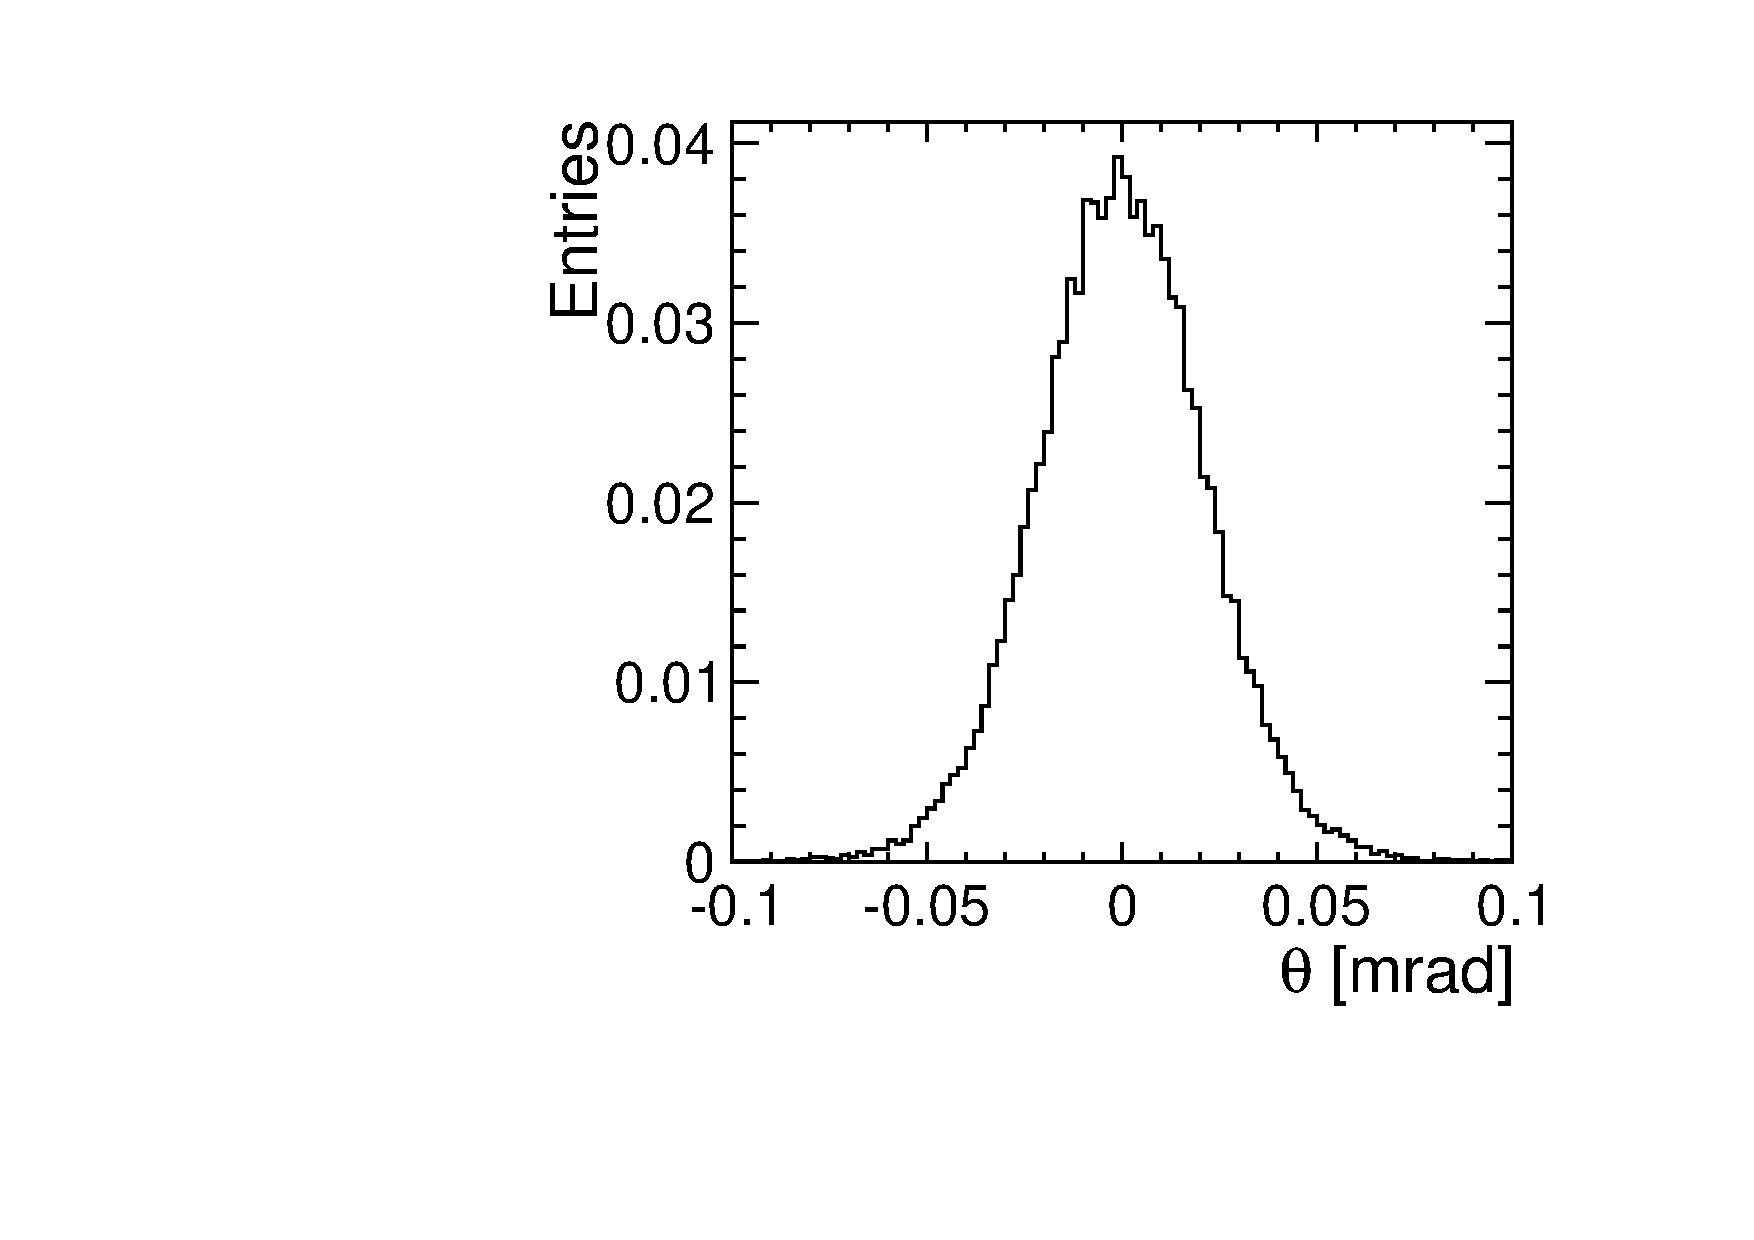
\includegraphics[width=\textwidth]{./figures/Telescope/MC_trackAngleTheta_planes_302_100.pdf}
    \caption{}
  \end{subfigure}
  \caption{Beam angular distribution in \textsc{Geant4} simulations
(comparing the global positions on the second telescope plane and on
the DUT).}
  \label{fig:MCbeamAngleDistr}
\end{figure}

\subsection{Biased residuals on each telescope plane}

\subsubsection{Track vs. hit}
\subsubsection{Track vs. MC}
\subsubsection{Hit vs. MC}

\subsection{Unbiased resolution on the DUT}
\subsubsection{Track vs. hit}
\subsubsection{Track vs. MC}

Unbiased residuals on the DUT ($100\,\micron$ thick sensor) in the x
and y directions (the dependence on the x and y of the residual is not
yet corrected in this plot).

\begin{figure}[htbp] \centering
  \begin{subfigure}[b]{0.45\textwidth}
    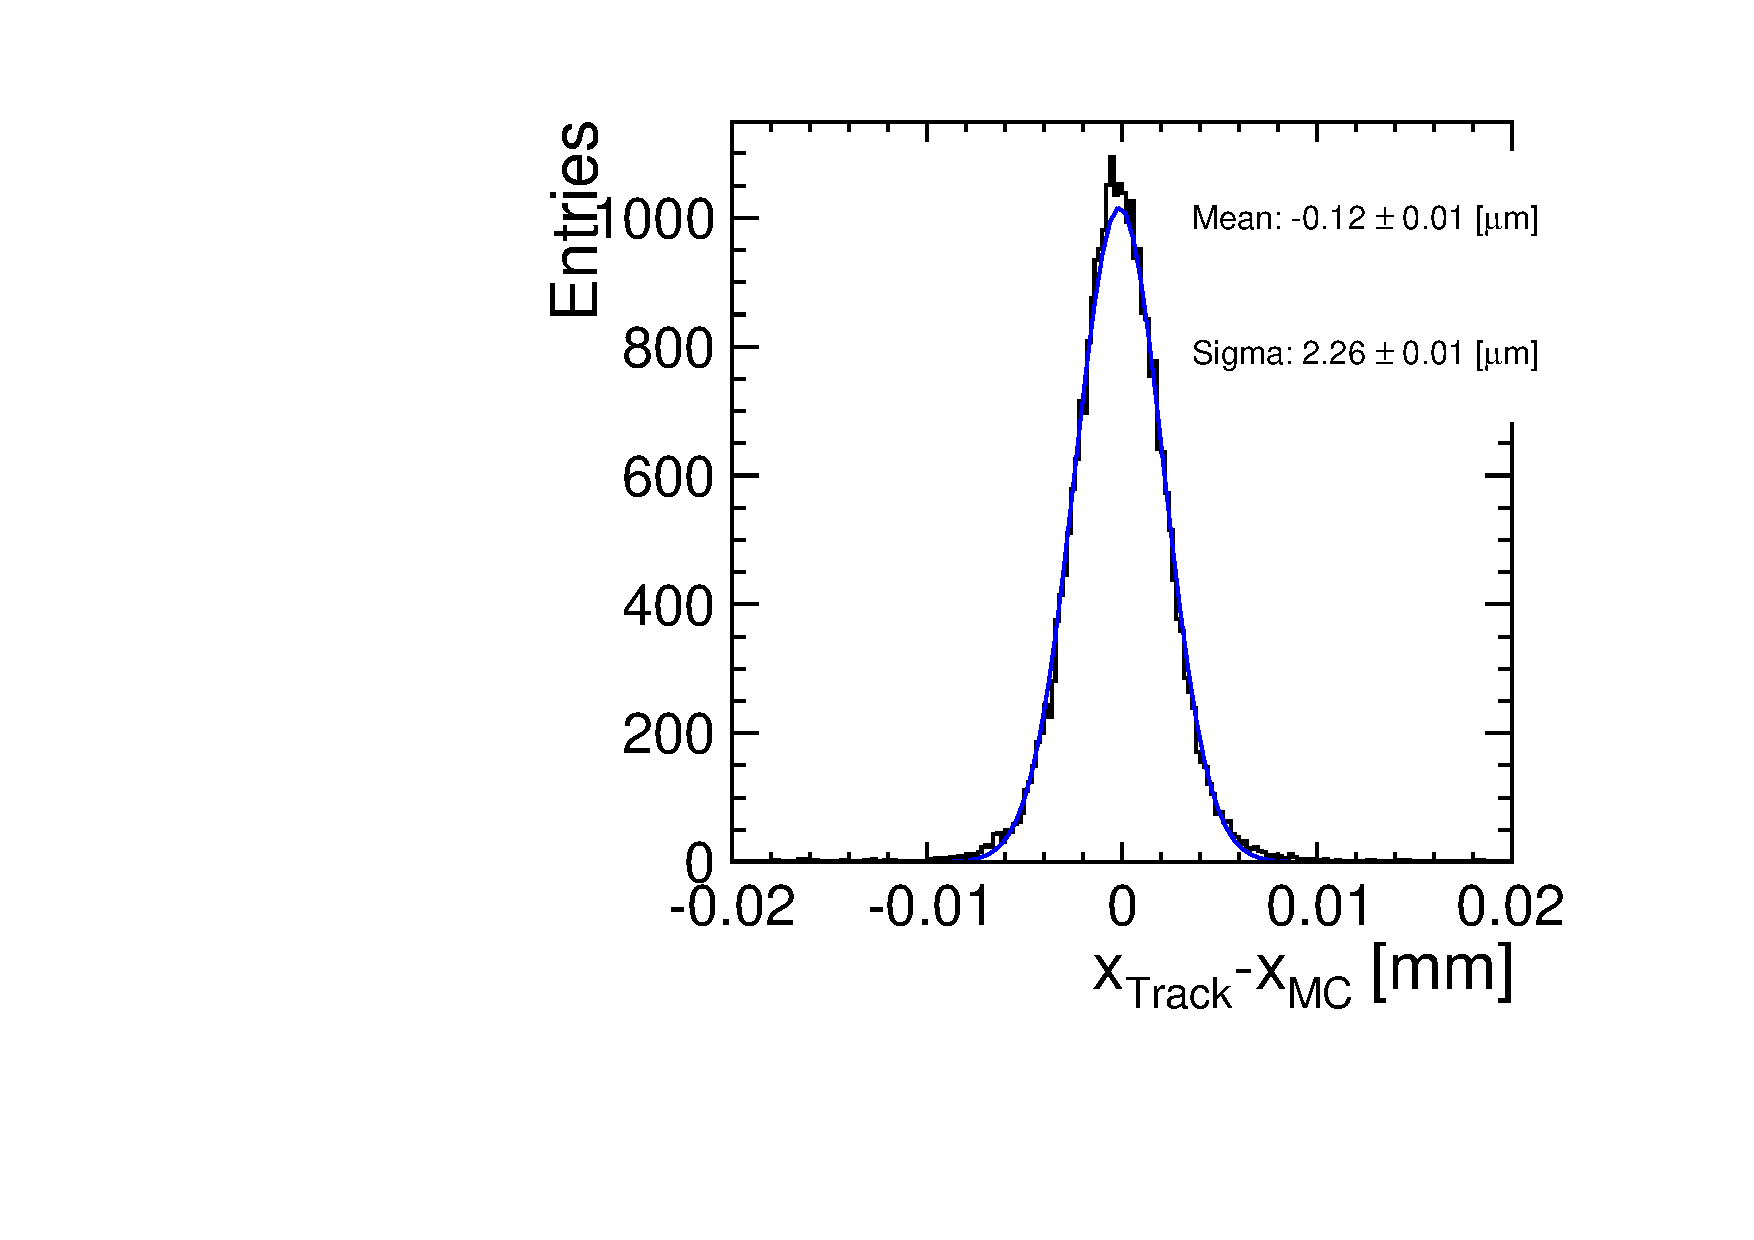
\includegraphics[width=\textwidth]{./figures/Telescope/run49_x_track_MC_DUT.pdf}
    \caption{}
  \end{subfigure}\hfill
  \begin{subfigure}[b]{0.45\textwidth}
    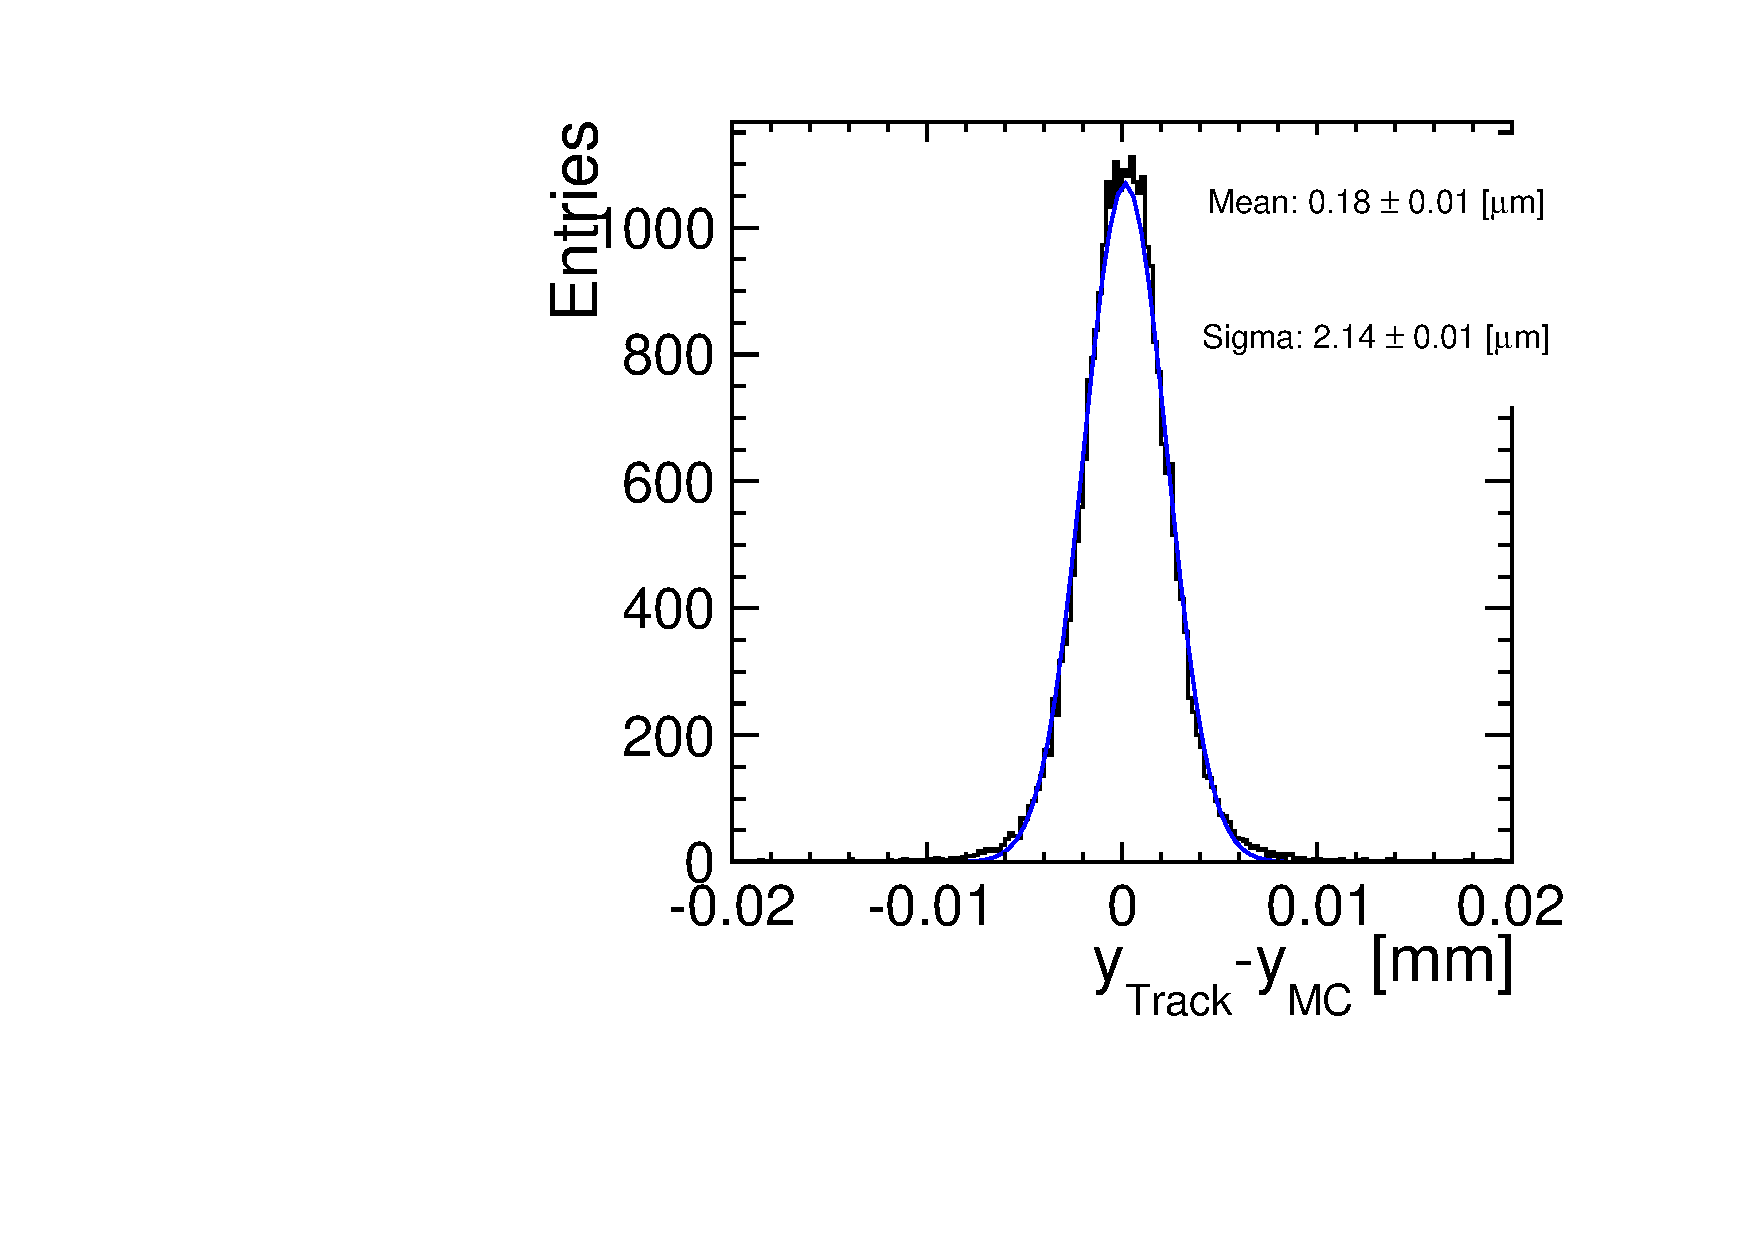
\includegraphics[width=\textwidth]{./figures/Telescope/run49_y_track_MC_DUT.pdf}
    \caption{}
  \end{subfigure}
  \caption{The tracking resolution on the DUT comparing the
    reconstructed track position to the true position of the particles
    coming from \textsc{Geant4}.}
  \label{fig:UnbiasedResidualOnDUT}
\end{figure}



\subsubsection{Hit vs. MC}

\subsection{Time stamping (?)}